\documentclass[a4paper]{article}

%% Language and font encodings
\usepackage[english]{babel}
\usepackage[utf8]{inputenc}
\usepackage{csquotes}
\bibliographystyle{unsrt}
\usepackage{booktabs}

\usepackage{tabu}
\usepackage[T1]{fontenc}

%% Sets page size and margins
\usepackage[a4paper,top=2cm,bottom=2cm,left=3cm,right=3cm,marginparwidth=1.75cm]{geometry}

%% Useful packages
\usepackage{amsmath}
\usepackage{graphicx}
%\usepackage{apacite}
\usepackage[colorinlistoftodos]{todonotes}
\usepackage[colorlinks=true, allcolors=blue]{hyperref}

\title {Simple Method of Improving Quarantine for CoronaVirus (COVID-2019) Through Location-Based Web-Services}
%\author{B. Shadrack Jabes}
\date{\it{\today}}

\begin{document}
\maketitle
                \begin{figure}
                \centering
                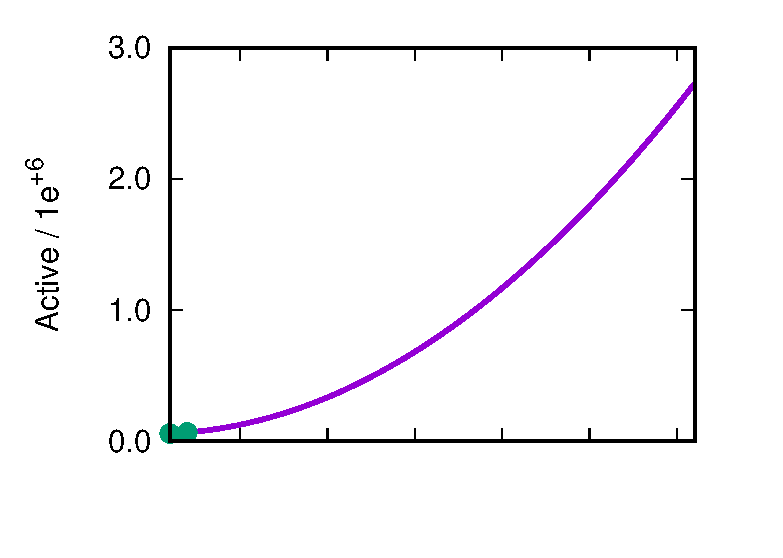
\includegraphics[clip=true,trim=0cm 0cm 0cm
                0cm,width=8cm]{ps.predict.active.ps}\\
			\vspace{-1.43cm}
                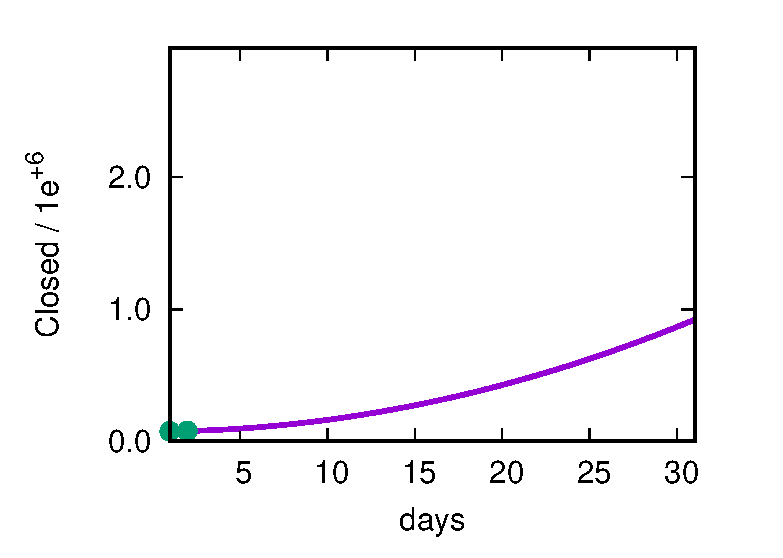
\includegraphics[clip=true,trim=0cm 0cm 0cm
                0cm,width=8cm]{ps.predict.closed.ps}
			\caption{The number of active (top) and closed (bottom) cases as a function of days. The dotted values shown in green represents the actual data and the violet line is the prediction. The functional form used is $f(x) = a_0 + a_1(x^2)$. The coefficients of the functional form for (top) are $a_0$ = 0.953233*$s_{active}$ and $a_1$ = 0.04676*$s_{active}$ and (bottom) are $a_0$ = 0.9885*$s_{closed}$ and $a_1$ = 0.0115*$s_{closed}$. Here, $s_{active}$ and $s_{active}$ are the number of active and closed cases on day 1 respectively. According to this model, the number of active cases in a month's time will be nearly 3 million and the closed clases will be 0.93 million.}
                \label{fig:fig1}
                \end{figure}
\end{document}
